\documentclass[12pt]{article}

\usepackage{amsmath, mathtools}
\usepackage{amsfonts}
\usepackage{amssymb}
\usepackage{graphicx}
\usepackage{colortbl}
\usepackage{xr}
\usepackage[destlabel]{hyperref}%inter-PDF linking with labels
\usepackage{longtable}
\usepackage{xfrac}
\usepackage{tabularx}
\usepackage{float}
\usepackage{siunitx}
\usepackage{booktabs}
\usepackage{caption}
\usepackage{pdflscape}
\usepackage{afterpage}

\usepackage[round]{natbib}

%\usepackage{refcheck}

\hypersetup{
%    bookmarks=true,         % show bookmarks bar?
      colorlinks=true,       % false: boxed links; true: colored links
    linkcolor=red,          % color of internal links (change box color with linkbordercolor)
    citecolor=green,        % color of links to bibliography
    filecolor=magenta,      % color of file links
    urlcolor=cyan           % color of external links
}

\input{../Comments}

% For easy change of table widths
\newcommand{\colZwidth}{1.0\textwidth}
\newcommand{\colAwidth}{0.13\textwidth}
\newcommand{\colBwidth}{0.82\textwidth}
\newcommand{\colCwidth}{0.1\textwidth}
\newcommand{\colDwidth}{0.05\textwidth}
\newcommand{\colEwidth}{0.8\textwidth}
\newcommand{\colFwidth}{0.17\textwidth}
\newcommand{\colGwidth}{0.5\textwidth}
\newcommand{\colHwidth}{0.28\textwidth}

% Used so that cross-references have a meaningful prefix
\newcounter{defnum} %Definition Number
\newcommand{\dthedefnum}{GD\thedefnum}
\newcommand{\dref}[1]{GD\ref{#1}}
\newcounter{datadefnum} %Datadefinition Number
\newcommand{\ddthedatadefnum}{DD\thedatadefnum}
\newcommand{\ddref}[1]{DD\ref{#1}}
\newcounter{theorynum} %Theory Number
\newcommand{\tthetheorynum}{T\thetheorynum}
\newcommand{\tref}[1]{T\ref{#1}}
\newcounter{tablenum} %Table Number
\newcommand{\tbthetablenum}{T\thetablenum}
\newcommand{\tbref}[1]{TB\ref{#1}}
\newcounter{assumpnum} %Assumption Number
\newcommand{\atheassumpnum}{P\theassumpnum}
\newcommand{\aref}[1]{A\ref{#1}}
\newcounter{goalnum} %Goal Number
\newcommand{\gthegoalnum}{P\thegoalnum}
\newcommand{\gsref}[1]{GS\ref{#1}}
\newcounter{instnum} %Instance Number
\newcommand{\itheinstnum}{IM\theinstnum}
\newcommand{\iref}[1]{IM\ref{#1}}
\newcounter{reqnum} %Requirement Number
\newcommand{\rthereqnum}{P\thereqnum}
\newcommand{\rref}[1]{R\ref{#1}}
\newcounter{lcnum} %Likely change number
\newcommand{\lthelcnum}{LC\thelcnum}
\newcommand{\lcref}[1]{LC\ref{#1}}

\newcommand{\famname}{rkf45 Generator} % PUT YOUR PROGRAM NAME HERE

\usepackage{fullpage}
\usepackage{tikz}
\usetikzlibrary{arrows}

\begin{document}

\title{RK Generator} 
\author{Alexander Schaap}
\date{\today}

\maketitle

~\newpage

\pagenumbering{roman}

\section{Revision History}

\begin{tabularx}{\textwidth}{p{3cm}p{2cm}X}
\toprule {\bf Date} & {\bf Version} & {\bf Notes}\\
\midrule
\today & 1.0 & Initial version\\
\bottomrule
\end{tabularx}

~\newpage
	
\section{Reference Material}

This section records information for easy reference.

\subsection{Table of Units}

Since the application of this software is dependent on the program using the 
functions provided by this program family, no physical units are used 
throughout this document.

\subsection{Table of Symbols}\label{ssec:symbols}

The table that follows summarizes the symbols used in this document. As stated 
above, no physical units are associated with any of these.  The choice of 
symbols was made to be consistent with the 
literature describing ODEs.\footnote{Specifically, 
\cite{corless_graduate_2013}.}  The symbols are listed in alphabetical order.

\renewcommand{\arraystretch}{1.2}
%\noindent \begin{tabularx}{1.0\textwidth}{l l X}
\noindent \begin{longtable*}{l p{12cm}} \toprule
\textbf{symbol} & \textbf{description}\\
\midrule 
$\mathbb{C}$ & Complex numbers
\\ 
${\bf f}$ & ODE for which to solve
\\
$h$ & step size
\\ 
${\bf k}_{1..4}$ & intermediate variables in the RK4 method, similar to 
${\bf Y}_1$ \wss{I don't know what the subscript notation means here.  Do you
  have 4 vectors of $k$ values or one vector with 4 values?}
\\ 
$\mathbb{R}$ & Real numbers
\\ 
$t$ & an independent variable, commonly time
\\ 
$t_0$ & beginning of interval
\\ 
$t_N$ & end of interval
\\ 
$t_k$ & any $t$ on the interval $[t_0..t_N]$
\\ 
${\bf x(t)}$ & a function of $t$
\\ 
${\bf x}'$ & derivative of ${\bf x(t)}$ \wss{add: with respect to $t$}
\\ 
${\bf x}_0$ & initial values for ${\bf f}$
\\ 
${\bf x}_k$ & (numerical approximation of) a point on the solution for 
${\bf f}$
\\ 
${\bf Y}_1$ & intermediate variables in the RK2 method, similar to ${\bf 
k}_{1..4}$
\\
\bottomrule
\end{longtable*}

\subsection{Abbreviations and Acronyms}

\renewcommand{\arraystretch}{1.2}
\begin{tabular}{l l} 
  \toprule
  \textbf{symbol} & \textbf{description}\\
  \midrule 
  A & Assumption\\
  DD & Data Definition\\
  GD & General Definition\\
  GS & Goal Statement\\
  IM & Instance Model\\
  LC & Likely Change\\
  ODE & Ordinary Differential Equation\\
  PS & Physical System Description\\
  R & Requirement\\
  RK & Runge-Kutta\\
  RK2 & Second order Runge-Kutta method\\
  RK4 & Fourth order Runge-Kutta method\\
%  RKF45 & Runge-Kutta-Fehlberg method\\
  \famname{} & Family of programs based on the RK2 / RK4 method(s)\\
  SRS & Software Requirements Specification\\
  STEM & Science, Technology, Engineering \& Mathematics\\
  T & Theoretical Model\\
  \bottomrule
\end{tabular}\\

\newpage

\tableofcontents

~\newpage

\pagenumbering{arabic}

\section{Introduction}
%modelled after 3dfim+
This document provides an overview of the commonality analysis (CA) for the 
\famname{} program family. Members of program family are produced by a code 
generator. Generated members provide numerical approximations for given 
ordinary differential equations (ODEs) using Runge-Kutta (RK) methods. Most of 
the calculations happens during code generation, producing a different family 
member for each given combination of RK method, ODE, interval, step size, and 
initial values. 
%The family member presents the results in the form of a function that can be 
%called. 
The current section describes the purpose of this document, the scope of this 
family, the organization of the remainder of the document and the 
characteristics of the intended reader.

\subsection{Purpose of Document}
%modelled after 3dfim+
The main purpose of this document is to provide sufficient information to 
understand what the \famname{} is expected to do.
The goals and theoretical models used in the \famname{} are provided, as are 
assumptions and unambiguous definitions.
This document should ultimately aid the development of the software by 
specifying and constraining the design, and by providing a starting point for 
the creation of test cases.
It should also give developers maintaining and/or improving the software a 
better idea of what it should and should not do, though improvement could 
require them to update this document.
For users (i.e. developers looking to incorporate this into their own 
software), this document details the uses and limitations of the \famname{}.

\subsection{Scope of the Family}
%loosely modelled after 3dfim+
The responsibility of the family is solving the provided ODEs for given 
intervals, initial values and step sizes using the specified RK method. The 
user will have to ensure the RK method specified is appropriate for their 
particular problem(s), and they will have to ensure appropriate and correct 
input is provided (see \nameref{ssec:Assumptions}). 
Additionally, the user will also have to process the output appropriately.

\wss{Your scope should specify which kind of ODEs you solve.  Your software
  solves systems of first order ODEs.  You do not solve higher order ODEs,
  presumably because they can be recast as systems of first order ODEs.  In
  addition, the functional form of your ODE can be given explicitly, as opposed
  to being in implicit form.}

\subsection{Characteristics of Intended Reader} 
The reader is expected to have some undergraduate background in a math-heavy 
science or engineering, as well as code generation. Ideally, they have been 
exposed to some undergraduate calculus courses that covered numerical methods 
for ODE's.
Programming courses would also help, especially some understanding of 
functional programming and metaprogramming. 
Metaprogramming may be beyond the scope of most undergraduate degrees though.
\wss{For the characteristics of intended reader try to be
  more specific about the education.  What degree?  What course areas?  What
  level?}
\als{I've tried to add some detail.}

\subsection{Organization of Document}
%inspired by FamilyOfMaterialModels
The organization of this document follows the template for a commonality 
analysis (CA) provided by Dr.~W.~S.~Smith, \wss{The citations are enough; you
  don't need to mention me separately} which is in turn adapted from 
\cite{Lai2004},\cite{SmithAndLai2005}, \cite{Smith2006} and 
\cite{SmithEtAl2007}.

The structure of this document is essentially top-down, with detail added as 
one proceeds through it. A general system description is provided first, 
followed by commonalities and variabilities. References are listed at the end.

\section{General System Description}

This section identifies the interfaces between the system and its environment,
describes the potential user characteristics and lists the potential system
constraints.

\subsection{Potential System Contexts}

\autoref{fig:systemcontext} shows the system context. A circle represents than 
external entity outside the software, which is the ``user'', or parent program 
making use of the generator as a library. A rectangle is used to represent the 
generator as well as the \famname{} family members it can generate. 

Ideally, 
the parent program knows the ODE(s) and other inputs at compile time, and
uses each generated family member many times at run-time to maximize the 
benefit of code generation. 
Alternatively, the ODE(s) or other inputs are 
not known at compile time; code generation can still happen at run-time, but 
hopefully the parent program can offset the incurred cost of this on-the-fly 
generation by running the optimized generated code enough times.

\begin{figure}[ht]
    \centering
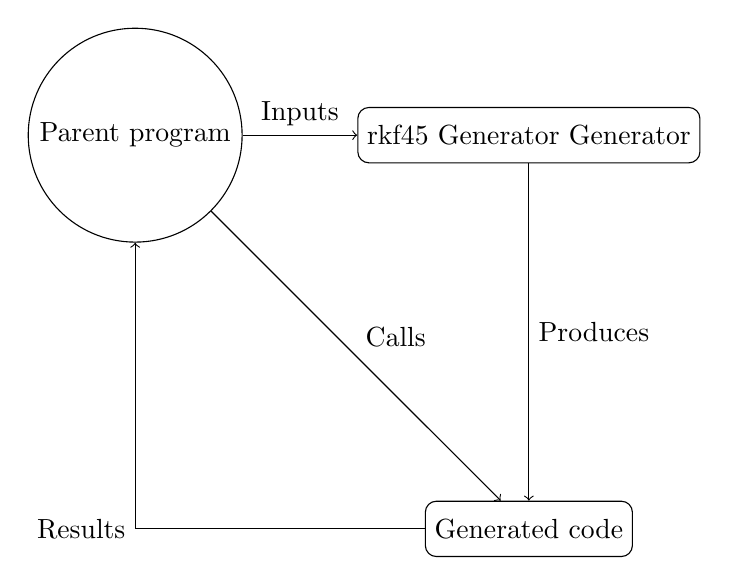
\begin{tikzpicture} [
    auto,
    c/.style = {circle, draw, text centered},
    b/.style = {rectangle, draw, text centered, rounded corners, minimum 
    height=2em},
    arrow/.style = {draw, ->},
    node distance = 5cm
    ]
    \node[c](user) {Parent program};
    \node[b, right of=user](RKgen) {\famname{} Generator}; 
    \node[b, below of=RKgen](gen) {Generated code};
    
    \draw[arrow] (user) -- node {Inputs} (RKgen);
    \draw[arrow] (RKgen) -- node {Produces} (gen);
    \draw[arrow] (user) -- node {Calls} (gen);
    \draw[arrow] (gen) -| node {Results} (user);
    
\end{tikzpicture}
\caption{System Context}
\label{fig:systemcontext}
\end{figure}

\begin{itemize}
\item User Responsibilities:
\begin{itemize}
\item Provide appropriate input to the system
\item Ensure assumptions on the input are met (see \autoref{ssec:Assumptions})
\item Correctly process the resulting output
\end{itemize}
\item \famname{} Responsibilities:
\begin{itemize}
\item Calculate the correct output for the given input
\end{itemize}
\end{itemize}

\subsection{Potential User Characteristics} \label{SecUserCharacteristics}

The most common user of \famname{} will be other programs. However, one or more 
programmers are needed to write the code that calls the functions provided by 
this family.
These programmers therefore should have an understanding of undergraduate 
calculus and OCaml programming. (Knowledge of MetaOCaml should not be necessary 
if the program family is able to hide its usage thereof sufficiently).
                                                                                
                          
\subsection{Potential System Constraints}

The responsibility of generating family members in a type-safe way restricts 
the system to the MetaOCaml extension of the OCaml programming language.
Code generation errors can be tricky (think C++ templates), so using a 
type-safe language ensures that if it compiles, it most likely works as 
expected.
This also helps avoid more subtle errors that could easily go unnoticed.
Alternatives tend to make less guarantees about the generated code.
\section{Commonalities}

This section contains the commonalities between the \famname{} family members. 
This section starts with succinct background information about the problem, 
followed by terminology and definitions, data definitions, goal statements and 
ending with theoretical models. 

\subsection{Background Overview} \label{Sec_Background}

There are various numerical methods for approximating ordinary differential 
equation (ODE) given initial values. This problem is called an initial value 
problem (IVP, see \tref{T_IVP}). A well-known way to solve these problems is 
through Runge-Kutta methods.% (which include Euler's method).

\subsection{Terminology and  Definitions}

This subsection provides a list of terms that are used in the subsequent
sections and their meaning, with the purpose of reducing ambiguity and making it
easier to correctly understand the requirements:

\begin{itemize}

\item Code generation: producing code programmatically.

\item Compile-time: the time during which a program is compiled.

\item Continuous function: a function that evaluates to a value that is not 
infinity or undefined for any input.

\item Initial value problem (IVP): an ODE along with initial values for which a 
numerical approximation must be found.

\item Initial values (initial condition): a starting point from which the rest 
of the approximation 
can be calculated. (See \ddref{DD_initialvalues}.)

\item Interval: interval inside which the ODE needs to be approximated. (See 
\ddref{DD_interval}.)

\item MetaOCaml: an extension to the OCaml programming language which adds 
staging annotations that enable MSP.

\item Metaprogramming: programming software that takes in and/or produces 
programs.

\item Multi-stage programming (MSP): a form of metaprogramming where the 
execution of specific code fragments is delayed; these fragments are then 
combined into larger fragments and ultimately executed.

\item OCaml: A multi-paradigm programming language (imperative \& functional) 
with a syntax that will appear somewhat unusual to most.

\item Ordinary differential equation (ODE): an equation that involves some 
ordinary (rather than partial) derivatives of a function. The goal is to find 
the function that satisfies the equation, and this is not always easily 
achievable through integration. (See \ddref{DD_ODE}.)

\item Runge-Kutta methods: a set of methods that approximate ODEs in IVPs for a 
given interval and step size.

\item Run-time: the time during which a program is run.

\item Step size: the distance between any two points for which to find 
approximations; it essentially determines how many points there will be once 
the interval is known. Once these points have been approximated, one could 
interpolate so that the whole interval is solved for. (See also 
\ddref{DD_stepsize}.)

\item Stiff ODE: an ODE for which certain numerical methods are numerically 
unstable unless the step size is extremely small. There is no exact definition.

\end{itemize}

\subsection{Data Definitions} \label{sec_datadef}

This section collects and defines all the data needed to build the instance
models. The dimension of each quantity is also given.
~\newline

\noindent
\begin{minipage}{\textwidth}
\renewcommand*{\arraystretch}{1.5}
\begin{tabular}{| p{\colAwidth} | p{\colBwidth}|}
\hline
\rowcolor[gray]{0.9}
Number& DD\refstepcounter{datadefnum}\thedatadefnum \label{DD_ODE}\\
\hline
Label& \bf Ordinary Differential Equation (ODE)\\
\hline
Symbol &${\bf f}$\\
\hline
 Units& N/A\\
 \hline
%  SI Units & \si{\watt\per\square\metre}\\
%  \hline
  Equation&${\bf x'} = {\bf f} (t,{\bf x} (t))$\\
  \hline
  Description & 
                 ${\bf f} : \mathbb{R} \times \mathbb{C}^n \rightarrow 
                 \mathbb{C}^n$ is the equation for which we ultimately want to 
                 find 
                 a numerical approximation. \wss{I don't think this is true.
                You know $f$ and you are trying to find $x$.}
  \\
  \hline
  Sources & \cite{corless_graduate_2013} \\
  \hline
  Ref.\ By & \iref{T_RK4}, \iref{IM_RK2}, \tref{T_IVP}\\
  \hline
\end{tabular}
\end{minipage}\\

~\newline

\noindent
\begin{minipage}{\textwidth}
    \renewcommand*{\arraystretch}{1.5}
    \begin{tabular}{| p{\colAwidth} | p{\colBwidth}|}
        \hline
        \rowcolor[gray]{0.9}
        Number& DD\refstepcounter{datadefnum}\thedatadefnum 
        \label{DD_interval}\\
        \hline
        Label& \bf Interval\\
        \hline
        Symbol &$t_0, t_N$\\
        \hline
        Units& N/A\\
        \hline
        %  SI Units & \si{\watt\per\square\metre}\\
        %  \hline
        Equation& N/A\\%all $ t \in [t_0, t_N]$\\
        \hline
        Description & 
        $[t_0,t_N] : \mathbb{R} \times \mathbb{R}$ is the interval for which to 
        solve the ODE (see \ddref{DD_ODE}). $t_0$ 
        represents the beginning of the interval, $t_N$ the end.
        \\
        \hline
  Sources & \cite{corless_graduate_2013} \\
  \hline
  Ref.\ By & \iref{T_RK4}, \iref{IM_RK2}\\
        \hline
    \end{tabular}
\end{minipage}\\

~\newline

\noindent
\begin{minipage}{\textwidth}
    \renewcommand*{\arraystretch}{1.5}
    \begin{tabular}{| p{\colAwidth} | p{\colBwidth}|}
        \hline
        \rowcolor[gray]{0.9}
        Number& DD\refstepcounter{datadefnum}\thedatadefnum 
        \label{DD_initialvalues}\\
        \hline
        Label& \bf Initial values\\
        \hline
        Symbol & ${\bf x}_0$\\
        \hline
        Units& N/A\\
        \hline
        %  SI Units & \si{\watt\per\square\metre}\\
        %  \hline
        Equation& ${\bf x}(t_0) = {\bf x}_0$\\
        \hline
        Description & 
        ${\bf x}_0 : \mathbb{C}^n$ are initial values for solving ODE (see 
        \ddref{DD_ODE}).
        \\
        \hline
  Sources & \cite{corless_graduate_2013} \\
  \hline
  Ref.\ By & \ddref{DD_stepsize}, \iref{T_RK4}, \iref{IM_RK2}, \tref{T_IVP}\\
        \hline
    \end{tabular}
\end{minipage}\\

~\newline

\noindent
\begin{minipage}{\textwidth}
    \renewcommand*{\arraystretch}{1.5}
    \begin{tabular}{| p{\colAwidth} | p{\colBwidth}|}
        \hline
        \rowcolor[gray]{0.9}
        Number& DD\refstepcounter{datadefnum}\thedatadefnum 
        \label{DD_stepsize}\\
        \hline
        Label& \bf Step size\\
        \hline
        Symbol & $h$ \\
        \hline
        Units& N/A \\
        \hline
        %  SI Units & \si{\watt\per\square\metre}\\
        %  \hline
        Equation& $t_{k+1} - t_k = h$\\
        \hline
        Description & 
        $h : \mathbb{R}$ is the distance between the points within interval 
        $[t_0,t_N]$ for which to find approximations.  %using RK methods (as 
        %described in 
        %\iref{T_RK4} and \iref{IM_RK2}).
        \\
        \hline
  Sources & \cite{corless_graduate_2013} \\
  \hline
  Ref.\ By & \iref{T_RK4}, \iref{IM_RK2}\\
        \hline
    \end{tabular}
\end{minipage}\\

\subsection{Goal Statements}

\noindent Given the non-stiff continuous ODE, the goal statements are:

\begin{itemize}

\item[GS\refstepcounter{goalnum}\thegoalnum \label{G_meaningfulLabel}:] Given 
an RK method specification, an interval and the desired step size, as well as 
an initial value, calculate a spline and generate (in a type-safe manner) a 
function that uses this spline to solve for specific points within the provided 
interval.

\end{itemize}

\wss{Why are you mentioning a spline?  In addition to solving the ode at the
  specified points, are you interpolating between the points using a spline?  If
  so, you should add information defining a spline, and you'll need to be more
  specific on what spline you are using in terms of order and continuity
  conditions at the knots.}

\subsection{Theoretical Models} \label{sec_theoretical}

This section focuses on the general equations and laws that \famname{} is based
on.

~\newline

\noindent
\begin{minipage}{\textwidth}
\renewcommand*{\arraystretch}{1.5}
\begin{tabular}{| p{\colAwidth} | p{\colBwidth}|}
  \hline
  \rowcolor[gray]{0.9}
  Number& T\refstepcounter{theorynum}\thetheorynum \label{T_IVP}\\
  \hline
  Label&\bf Initial value problem (IVP)\\
  \hline
  Equation&  ${\bf x'} = {\bf f} (t,{\bf x} (t))$, \quad ${\bf 
  x}(t_0) = {\bf x}_0$ \quad
    where 
    \begin{itemize}
        \item ${\bf x} : \mathbb{R} \rightarrow \mathbb{C}^n$ is the 
    vector solution as a function of time
        \item ${\bf x}_0 \in 
        \mathbb{C}^n$ is the initial condition (see \ddref{DD_initialvalues})
        \item ${\bf f} : 
    \mathbb{R} \times \mathbb{C}^n \rightarrow \mathbb{C}^n$ is the function 
    describing the vector field (see \ddref{DD_ODE})
   \end{itemize} 
   Given an initial value ${\bf x}_0$, the goal is to find approximations on a 
   given interval $[t_0 .. t_N]$.\\
  \hline
  Description & 
                The standard form of an initial value problem is given above. 
                The issue is that many IVPs are difficult to solve manually (or 
                programmatically) and the correct solutions are often unknown. 
                Numerical methods are close enough to be used in most 
                applications.\\
  \hline
  Source &
           \cite{corless_graduate_2013} p. 510, 513\\
  % The above web link should be replaced with a proper citation to a publication
  \hline
  Ref.\ By & \iref{T_RK4}, \iref{IM_RK2} \\
  \hline
\end{tabular}
\end{minipage}\\

\wss{It would be better if you used the instance model template for your
  theoretical model.  In particular, a clear separation between the inputs and
  the ouputs would be nice.}

\section{Variabilities}

Assumptions on all variations of the program family are covered first.
Variability in RK method in the \famname{} program family are represented by
instance models in \nameref{sec_Calculation}. Every unique input will result in
slightly different code being generated, which could in turn produce different
output compared to other family members. This allows for an infinite program
family depending on one's definition of program family\footnote{Currently
  Dr. Smith and Dr. Carette agree they should discuss this definition to compare
  their overlapping but slightly differing viewpoints. \wss{By default, LaTeX
    puts two spaces after a period, since it assumes that the period ends a
    sentence.  To override this, use x.\ y or x.~y.  The first puts one space,
    the second option also does one space, with the added constraint that a line
    break cannot happen at the space.}}. After instance models, the lack of
variability in output is covered.

\subsection{Assumptions}\label{ssec:Assumptions}

\begin{itemize}

\item[A\refstepcounter{assumpnum}\theassumpnum \label{A_RKorder}:] The user 
will specify what order of RK method they want used during code generation, 
either second (\iref{T_RK4}) or fourth (\iref{IM_RK2}). \wss{This is a
  variability, but it isn't an assumption.}

\item[A\refstepcounter{assumpnum}\theassumpnum 
\label{A_ODEnonstiffcontinuous}:] The ODE (\ddref{DD_ODE}) provided will be 
continuous and 
non-stiff (otherwise the user accepts that the results will be inaccurate)

\item[A\refstepcounter{assumpnum}\theassumpnum \label{A_initialvaluesata}:] The 
given initial values (\ddref{DD_initialvalues}) are for the beginning of the 
interval (\ddref{DD_interval}), represented by $t_0$. \wss{The assumptions don't
  need to repeat things you have alread said.}

\item[A\refstepcounter{assumpnum}\theassumpnum \label{A_initialvalues}:] 
Initial value (\ddref{DD_initialvalues}) vector size is expected to match the 
ones produced by the ODE 
(\ddref{DD_ODE}).

\item[A\refstepcounter{assumpnum}\theassumpnum \label{A_interval}:] The 
interval's bounds (\ddref{DD_interval}) satisfy $t_0 < t_N$ (both real 
numbers) and $t_N - t_0 = n 
\times h$. \wss{In general with floating point arithmetic this won't necessarily
  be true.  In practice if $h$ is added to the time for each time step, you
  won't end exactly at $t_N$.  Do you really need this assumption to be true?}

\item[A\refstepcounter{assumpnum}\theassumpnum \label{A_stepsize}:] The step 
size (\ddref{DD_stepsize}) shall be a positive real number. \wss{You can give
  this through the type of $h$; you don't need an assumption for this information.}

\end{itemize}

\wss{It is okay to have a short list of assumptions.  It feels like you might
  have been trying to ``pad'' the list.  What about an assumption that $f$ is
  continuous on the interval of computation?}

\subsection{Calculation} \label{sec_Calculation}

The family can utilize either of the instance models listed below for any of 
its members.

\wss{To make this clear that you have a family of methods, I would introduce an
  instance model for one-step initial value problem solvers.  The equation would
  be $${\bf x}_{k+1} = {\bf x}_k + h \phi(t_k, {\bf x}_k, h_k)$$  The only
  difference for your family members is how $\phi$ is defined.  This approach
  would let you easily add new family members in the specification, simply by
  giving new values for $\phi$.}

\noindent
\begin{minipage}{\textwidth}
    \renewcommand*{\arraystretch}{1.5}
    \begin{tabular}{| p{\colAwidth} | p{\colBwidth}|}
        \hline
        \rowcolor[gray]{0.9}
        Number& IM\refstepcounter{instnum}\theinstnum \label{T_RK4}\\
        \hline
        Label&\bf Fourth order Runge-Kutta method (RK4)\\
        \hline
        Equation&  
        \begin{itemize}
            \item $t_1 = t_0 + h$
            \item ${\bf k}_1 = {\bf f} (t_0, {\bf x}_0)$ slope at $x_0$
            \item ${\bf k}_2 = {\bf f} (t_0 + \dfrac{h}{2}, {\bf x}_0 + 
            \dfrac{h}{2} {\bf k}_1)$ slope of the point halfway between $t_0$ 
            and $t_1$ when extrapolating slope ${\bf k}_1$ from point ${\bf 
                x}_0$
            \item ${\bf k}_3 = {\bf f} (t_0 + \dfrac{h}{2}, {\bf x}_0 + 
            \dfrac{h}{2} {\bf k}_2)$ slope of the point halfway between $t_0$ 
            and $t_1$ when extrapolating slope ${\bf k}_2$ from point ${\bf 
                x}_0$
            \item ${\bf k}_4 = {\bf f} (t_0 + h, {\bf x}_0 + 
            h {\bf k}_3)$ slope of point at $t_1$ when extrapolating slope 
            ${\bf k}_3$ from point ${\bf x}_0$
            \item ${\bf x}_1 = {\bf x}_0 + \dfrac{h}{6} ( {\bf k}_1 + 2 {\bf 
                k}_2 + 2 {\bf k}_3 + {\bf k}_4)$ new point created when 
            extrapolating from point ${\bf x}_0$ using a weighted average of 
            the previously calculated slopes
            
        \end{itemize}\\
        \hline
        Description & 
        The above equations can be used to calculate (an approximation of) a 
        new point given the previous or starting point. Note that the above is 
        a specific instance (for simplicity) of the general method (namely, the 
        first step). \wss{Why specify the first step?  Why not specify the $k$th
                      step?}  Calculating a new point is necessary to create a spline to 
        solve IVPs (\tref{T_IVP}). In addition to the ODE (\ddref{DD_ODE}), 
        this 
        also requires an interval (\ddref{DD_interval}), step size 
        (\ddref{DD_stepsize}) and initial condition 
        (\ddref{DD_initialvalues}).\\
        \hline
        Source &
        \cite{corless_graduate_2013} p. 618\\
        % The above web link should be replaced with a proper citation to a 
        %publication
        \hline
        Ref.\ By & N/A\\
        \hline
    \end{tabular}
\end{minipage}\\

\wss{Again, I'm not sure how splines fit into this?}

~\newline
\noindent
\begin{minipage}{\textwidth}
    \renewcommand*{\arraystretch}{1.5}
    \begin{tabular}{| p{\colAwidth} | p{\colBwidth}|}
        \hline
        \rowcolor[gray]{0.9}
        Number & IM\refstepcounter{instnum}\theinstnum \label{IM_RK2}\\
        \hline
        Label &\bf Second-order Runge-Kutta method (Improved Euler method)\\
        \hline
        Equations &  
        \begin{itemize}
            \item ${\bf Y}_1 = {\bf x}_k + h {\bf f} (t_k, {\bf x}_k)$ %new 
            %intermediate point at x_{k+1} by extrapolating slope at x_k
            \item ${\bf x}_{k+1} = {\bf x}_k + h \Big( \dfrac{1}{2} {\bf f} 
            (t_k,{\bf x}_k) + \dfrac{1}{2} {\bf f} (t_{k+1}, {\bf Y}_1) \Big)$ 
            %new point by averaging slope at current point and slope at new 
            %point for extrapolating from current point
        \end{itemize}\\
        \hline
        Description & 
        The above equations can be used to calculate (an approximation of) a 
        new point given the previous or starting point. Calculating a new point 
        is necessary to create a spline to 
        solve IVPs (\tref{T_IVP}). In addition to the ODE (\ddref{DD_ODE}) this 
        also requires an interval (\ddref{DD_interval}), step size 
        (\ddref{DD_stepsize}) and initial condition 
        (\ddref{DD_initialvalues}).\\
        \hline
        Source &
        \cite{corless_graduate_2013} p. 616 \\
        % The above web link should be replaced with a proper citation to a 
        %publication
        \hline
        Ref.\ By & N/A\\
        \hline
    \end{tabular}
\end{minipage}\\

~\newline

\wss{Why isn't the function $f$ listed as a variability?  You get a different
  program depending on the value of $f$.}

\subsection{Output} \label{sec_Output}    
N/A. Every program family member will output a numerical approximation of an 
ODE in the form of a function that can be called by the user.

\section{Traceability Matrices and Graphs}
The traceability matrices below show the relationships between the various 
concepts defined in this document. Rows may be affected by changes in the items 
the columns consist of (especially in the context of assumptions.)
\begin{table}[ht]
  \centering
  \begin{tabular}{lccccccc}
  \toprule
    & \ddref{DD_ODE} & \ddref{DD_interval} & \ddref{DD_initialvalues} & 
    \ddref{DD_stepsize} & \tref{T_IVP} & \iref{T_RK4} & \iref{IM_RK2}  \\ 
    \midrule
\ddref{DD_ODE} &  &  &  &  & \checkmark &  &  \\ 
\ddref{DD_interval}    &  &  &  &  & \checkmark &  &  \\ 
\ddref{DD_initialvalues}    & \checkmark &  &  &  & \checkmark &  &  \\ 
\ddref{DD_stepsize}    &  & \checkmark &  &  & \checkmark &  &  \\ 
\tref{T_IVP}    &  &  &  &  &  &  &  \\ 
\iref{T_RK4}    & \checkmark & \checkmark & \checkmark & \checkmark & 
\checkmark &  &  \\ 
\iref{IM_RK2}    & \checkmark & \checkmark & \checkmark & \checkmark & 
\checkmark &  &  
\\ 
\bottomrule
\end{tabular}
\caption{Traceability matrix between instance models, data definitions and 
theory}
\end{table}

\begin{table}[ht]
  \centering
  \begin{tabular}{lcccccc}
  \toprule 
  & \aref{A_RKorder} & \aref{A_ODEnonstiffcontinuous} & 
  \aref{A_initialvaluesata} & \aref{A_initialvalues} 
  & \aref{A_interval} & \aref{A_stepsize} \\ 
  \midrule 
\ddref{DD_ODE} &  & \checkmark &  &  &  &  \\ 
\ddref{DD_interval} &  &  &  &  & \checkmark &  \\ 
\ddref{DD_initialvalues} &  &  & \checkmark & \checkmark &  &  \\ 
\ddref{DD_stepsize} &  &  &  &  &  & \checkmark \\ 
\tref{T_IVP} &  &  & \checkmark &  &  &  \\ 
\iref{T_RK4} & & \checkmark &  &  &  &  \\ 
\iref{IM_RK2} & & \checkmark &  &  &  &  \\ 
  \bottomrule 
\end{tabular}
\caption{Traceability matrix for assumptions}
\end{table}
\clearpage
\newpage

\bibliographystyle {plainnat}
\bibliography {../References,../ReferencesA}

%\newpage
%
%\section{Appendix}
%
%\wss{Your report may require an appendix.  For instance, this is a good point 
%to
%show the values of the symbolic parameters introduced in the report.}
%
%\subsection{Symbolic Parameters}
%
%\wss{The definition of the requirements will likely call for 
%SYMBOLIC\_CONSTANTS.
%Their values are defined in this section for easy maintenance.}

\end{document}